\subsection{Stéréovision.}
\begin{frame}
    \frametitle{Principe.}
    \begin{tabular}{cc}
        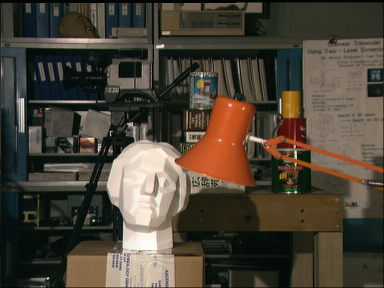
\includegraphics[width=.4\linewidth]{rcs/tsukuba.png} & 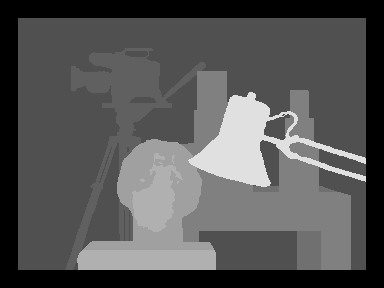
\includegraphics[width=.4\linewidth]{rcs/tsukuba_disp.png} \\
    \end{tabular}
    \only<2-3> { \begin{exampleblock}{Avantages}
            \begin{itemize}
                \pause \item Détecte tous les obstacles dans le champ de vision de la caméra.
                \pause \item Efficace contre les obstacles de type \emph{coin de table}.
            \end{itemize}
    \end{exampleblock} }
    \only<4-> { \begin{alertblock}{Limites}
            \begin{itemize}
                \pause \item Calculatoire et complexe.
                \pause \item Nécessite une unité de calcul puissante : coût élevé.
            \end{itemize}
    \end{alertblock} }
\end{frame}

\begin{frame}
    \frametitle{Résultats.}
    \begin{tabular}{ccc}
        \textbf{Caméra gauche} & \textbf{Caméra droite} & \textbf{Carte de disparité} \\
        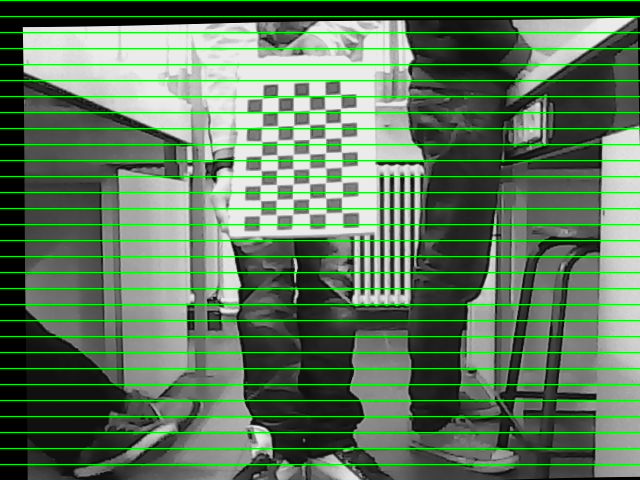
\includegraphics[width=0.3\linewidth]{rcs/rem0l.png} & 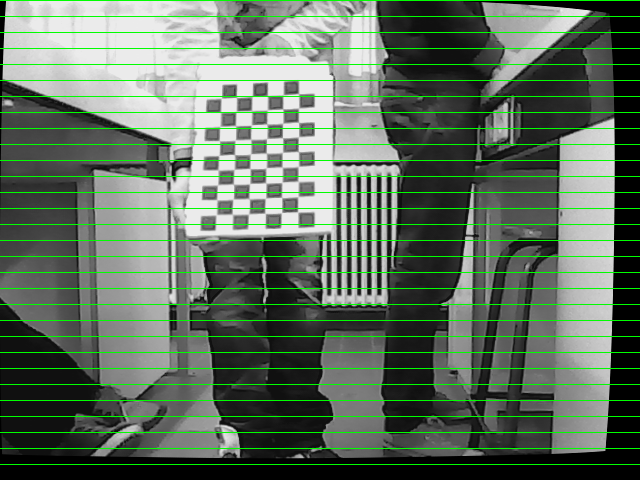
\includegraphics[width=0.3\linewidth]{rcs/rem0r.png} & 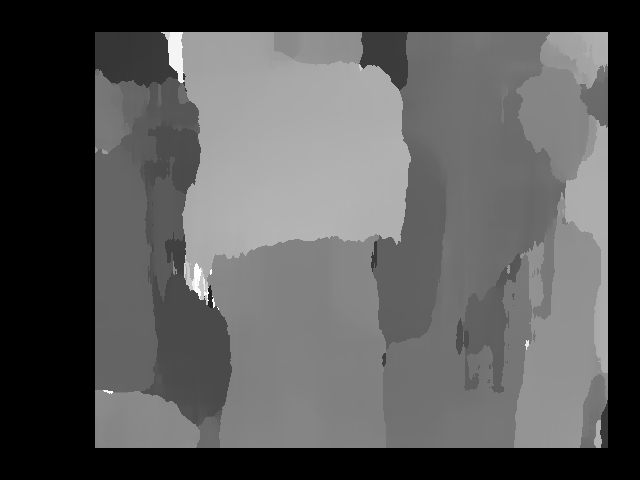
\includegraphics[width=0.3\linewidth]{rcs/disp0.png} \\
        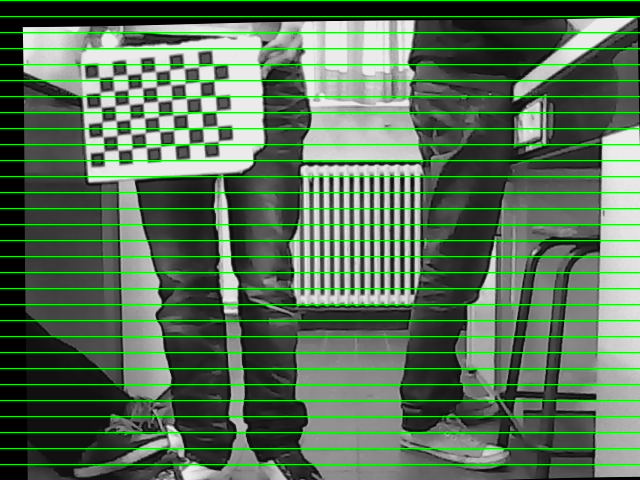
\includegraphics[width=0.3\linewidth]{rcs/rem1l.png} & 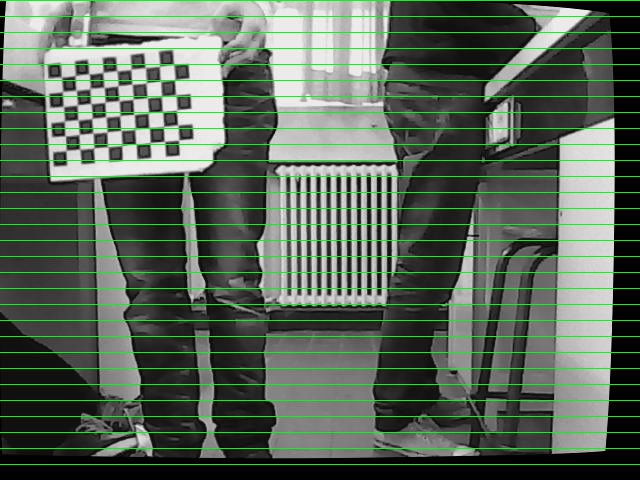
\includegraphics[width=0.3\linewidth]{rcs/rem1r.png} & 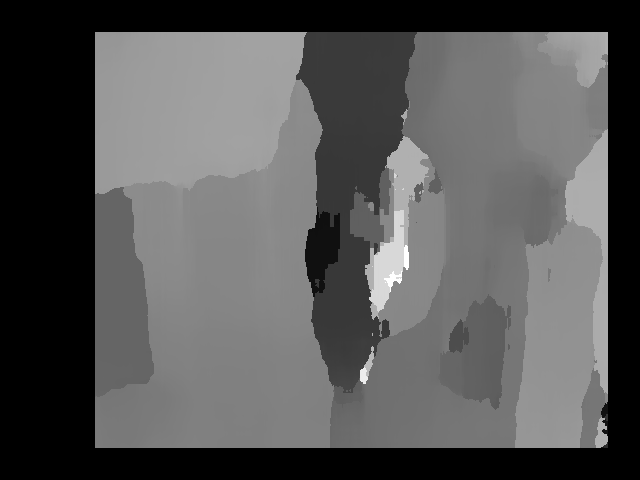
\includegraphics[width=0.3\linewidth]{rcs/disp1.png} \\
        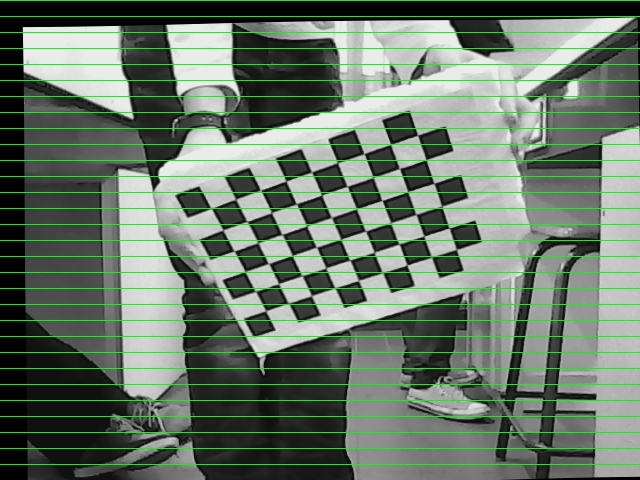
\includegraphics[width=0.3\linewidth]{rcs/rem2l.png} & 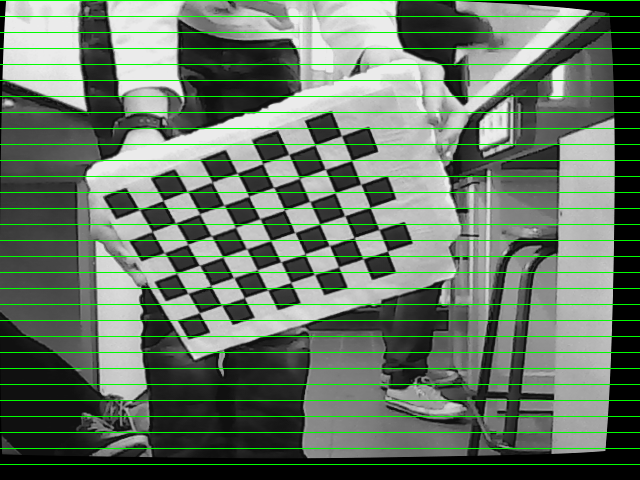
\includegraphics[width=0.3\linewidth]{rcs/rem2r.png} & 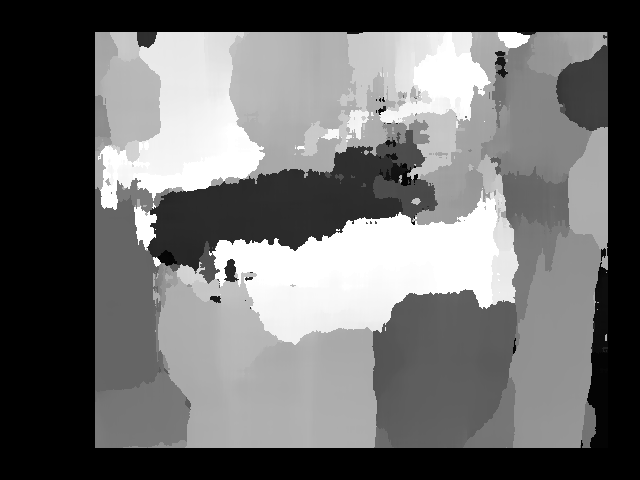
\includegraphics[width=0.3\linewidth]{rcs/disp2.png} \\
    \end{tabular}
\end{frame}

\subsection[ABOD]{Approche ABOD.}
\begin{frame}
    \frametitle{Principe.}
    \only<1> {
        \begin{center}
            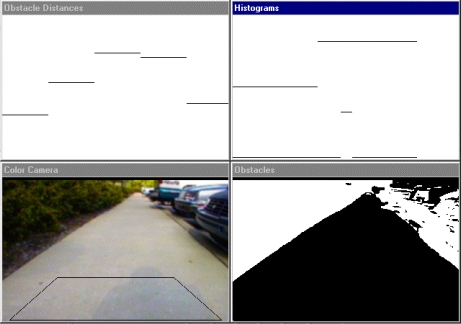
\includegraphics[width=0.8\linewidth]{rcs/abod.png}
        \end{center}
    }
    \only<2-> {
        \begin{alertblock}{Limites}
            \begin{itemize}
                \pause \item Le sol doit être globalement uni et différent des obstacles.
                \pause \item Inefficace contre les obstacles de type \emph{coin de table}.
                \pause \item Sans être aussi calculatoire que la stéréovision, nécessite une unité de calcul puissante.
                \pause \item A une période d'apprentissage : ne peut pas fonctionner dans un environnement inconnu.
            \end{itemize}
        \end{alertblock}
    }
\end{frame}

\begin{frame}
    \frametitle{Simulation.}
    \begin{center}
        \only<1> {
            \begin{tabular}{cc}
                \textbf{Caméra} & \textbf{Résultat} \\
                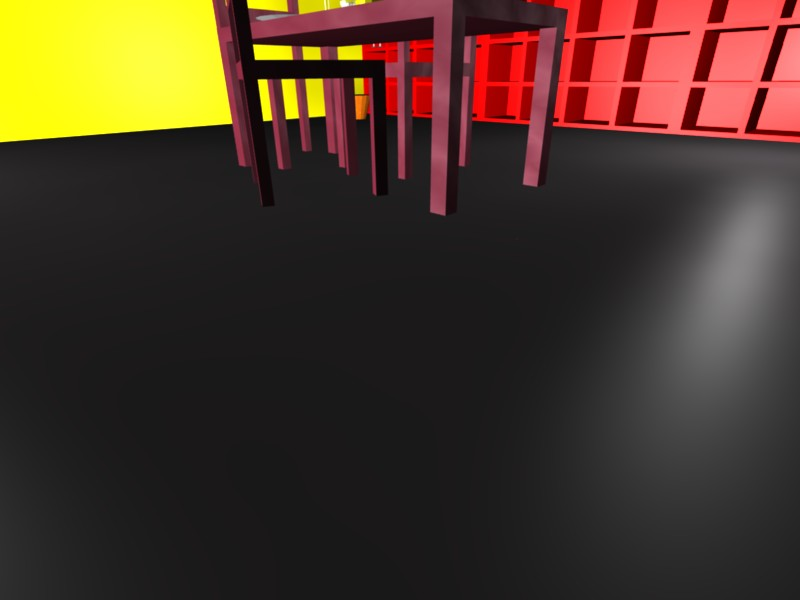
\includegraphics[width=0.4\linewidth]{rcs/abodv0s.png} & 
\includegraphics[width=0.4\linewidth]{rcs/abodv0r.png} \\
            \end{tabular}
            \begin{block}{Détails}
                \begin{itemize}
                    \item Indique $75\%$ de sol alors qu'il y en a $76.5\%$ : $1.7\%$  du sol est annoncé comme obstacle.
                    \item Indique $25\%$ d'obstacles alors qu'il y en a $23.5\%$ : $0.1\%$ des obstacles sont anoncés comme faisant partie du sol.
                \end{itemize}
            \end{block}
        } \only<2> {
            \begin{tabular}{cc}
                \textbf{Caméra} & \textbf{Résultat} \\
                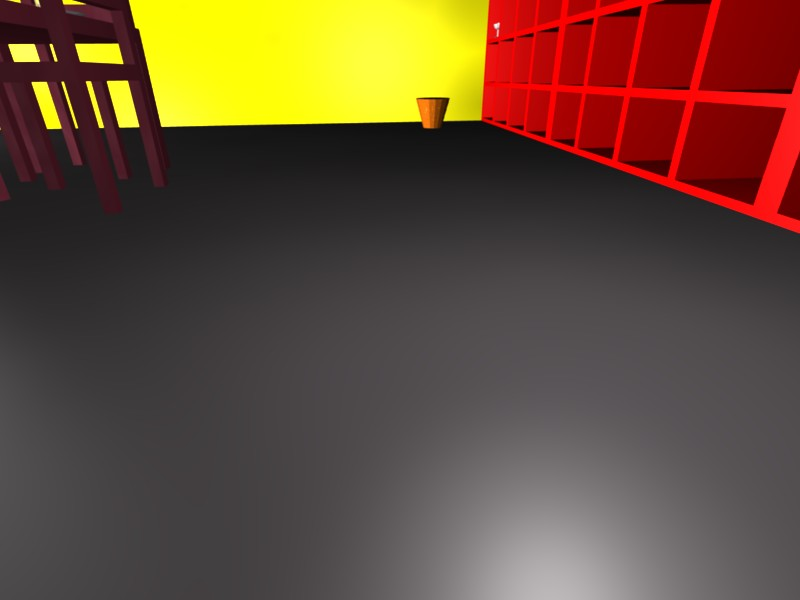
\includegraphics[width=0.4\linewidth]{rcs/abodv1s.png} & 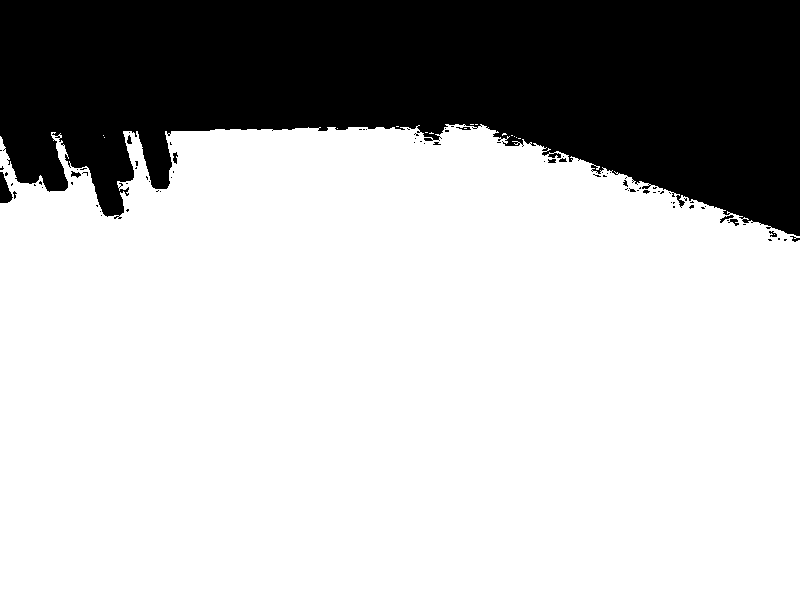
\includegraphics[width=0.4\linewidth]{rcs/abodv1r.png} \\
            \end{tabular}
            \begin{block}{Détails}
                \begin{itemize}
                    \item Indique $73\%$ de sol alors qu'il y en a $74.4\%$ : $1.7\%$  du sol est annoncé comme obstacle.
                    \item Indique $27\%$ d'obstacles alors qu'il y en a $25.6\%$ : tous les obstacles sont anoncés comme tel.
                \end{itemize}
            \end{block}
        } \only<3> {
            \begin{tabular}{cc}
                \textbf{Caméra} & \textbf{Résultat} \\
                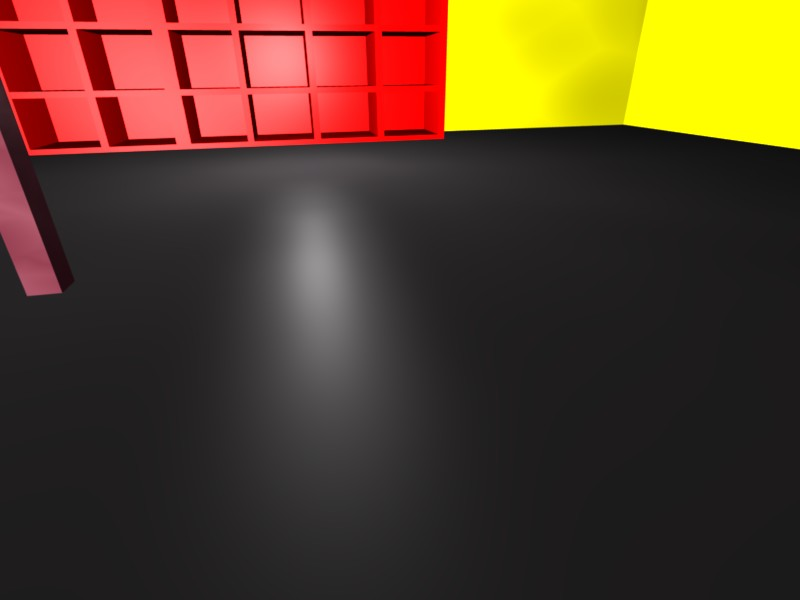
\includegraphics[width=0.4\linewidth]{rcs/abodv2s.png} & 
\includegraphics[width=0.4\linewidth]{rcs/abodv2r.png} \\
            \end{tabular}
            \begin{block}{Détails}
                \begin{itemize}
                    \item Indique $74.1\%$ de sol alors qu'il y en a $75.1\%$ : tout le sol est annoncé comme tel.
                    \item Indique $25.9\%$ d'obstacles alors qu'il y en a $24.9\%$ : $1.2\%$ des obstacles sont anoncés comme faisant partie du sol.
                \end{itemize}
            \end{block}
        }
    \end{center}
\end{frame}

\begin{frame}
    \frametitle{Résultats.}
    \begin{center}
        \only<1> {
            \begin{tabular}{cc}
                \textbf{Caméra} & \textbf{Résultat} \\
                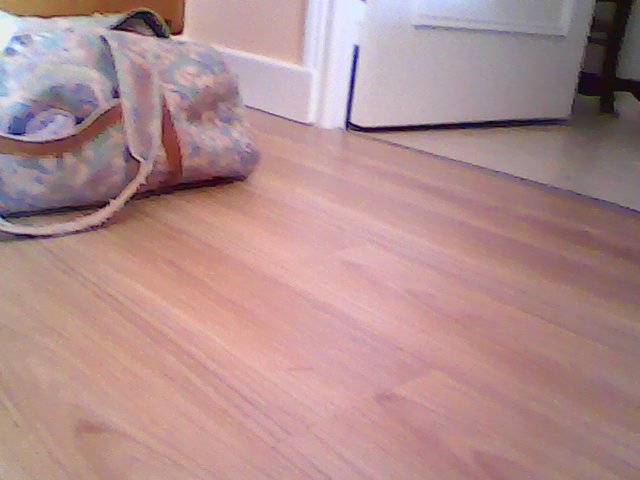
\includegraphics[width=0.4\linewidth]{rcs/abodr0s.png} & 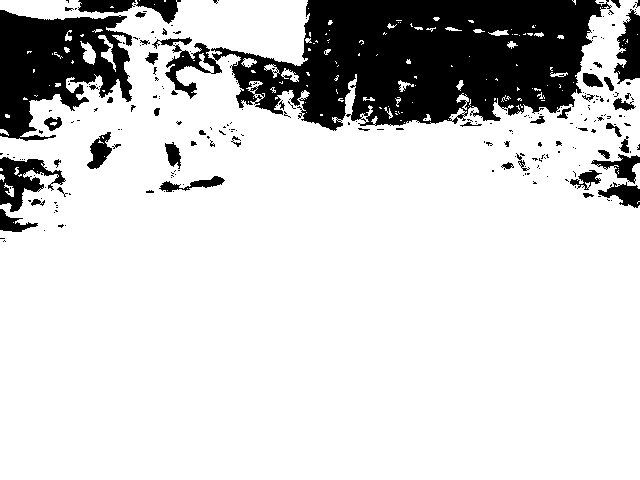
\includegraphics[width=0.4\linewidth]{rcs/abodr0r.png} \\
            \end{tabular}
            \begin{block}{Détails}
                \begin{itemize}
                    \item Indique $82\%$ de sol alors qu'il y en a $62.6\%$ : tout le sol est annoncé comme tel.
                    \item Indique $18\%$ d'obstacles alors qu'il y en a $37.4\%$ : $51.8\%$ des obstacles sont anoncés comme faisant partie du sol.
                \end{itemize}
            \end{block}
        } \only<2> {
            \begin{tabular}{cc}
                \textbf{Caméra} & \textbf{Résultat} \\
                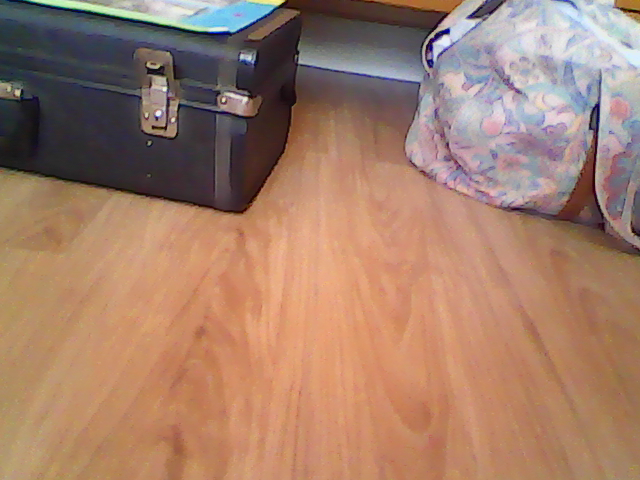
\includegraphics[width=0.4\linewidth]{rcs/abodr1s.png} & 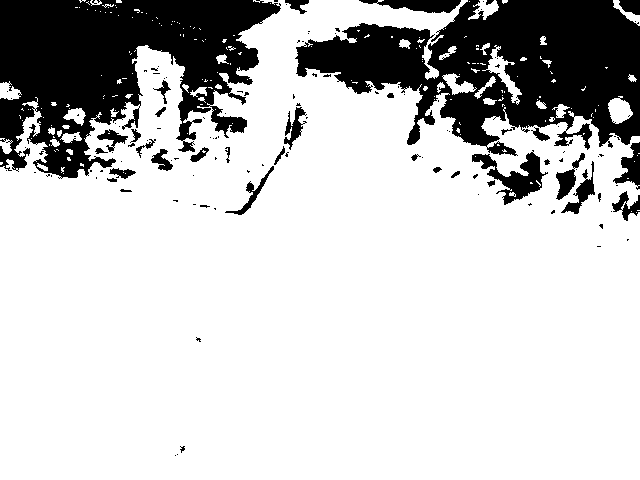
\includegraphics[width=0.4\linewidth]{rcs/abodr1r.png} \\
            \end{tabular}
            \begin{block}{Détails}
                \begin{itemize}
                    \item Indique $78.3\%$ de sol alors qu'il y en a $63.4\%$ : $0.7\%$  du sol est annoncé comme obstacle.
                    \item Indique $21.7\%$ d'obstacles alors qu'il y en a $36.6\%$ : $41.9\%$ des obstacles sont anoncés comme faisant partie du sol.
                \end{itemize}
            \end{block}
        }
    \end{center}
\end{frame}

